\section{Polyglot files via Encryption}

Using the same techniques, either using comments, metadata, or custom sections, it is also possible to hide files within other files, 
but instead of storing the raw contents of the hidden file, we can transform the contents of the hidden file using other means, such as encryption.

To demonstrate this we'll create a PDF that when decrypted using CBC mode with the block cipher AES with the right key and IV it will convert to a valid WASM binary.

CBC mode when encrypting XORs the current block with the previous block, in case its the first block it uses the IV, and then proceeds to encrypt the result
under the given key. The decryption is the exact opposite, we take the ciphertext block decrypt it under the key and then XOR the previous block, in case of the first block
the IV is used, the process is depicted by the following two pictures.

\begin{figure}[h]
    \center
    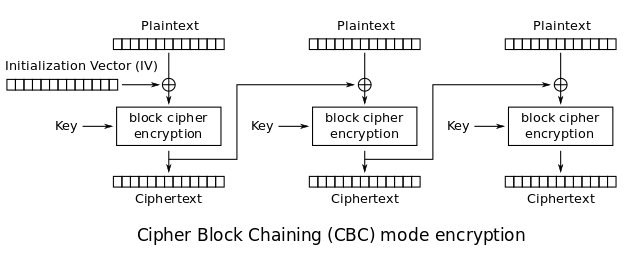
\includegraphics[width=8cm]{images/encryption.png}
    \caption{CBC encryption\cite{cbc}}
\end{figure}

\begin{figure}[h]
    \center
    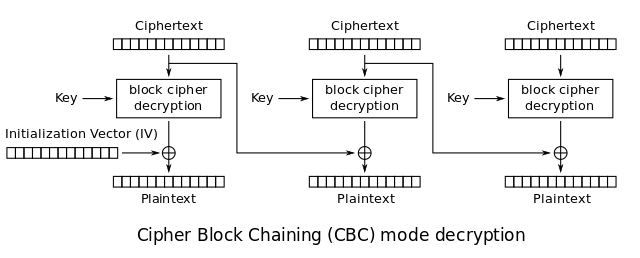
\includegraphics[width=8cm]{images/decryption.png}
    \caption{CBC decryption\cite{cbc}}
\end{figure}

We can't really do much with controlling the output as changing only a single byte results in a completely different sequence of bytes. What we can do here
is control the first block and the IV.

We need to create an IV that when used with a CBC block mode cipher, it decrypts a PDF header into parts of valid WASM binary. We can actually construct
such IV with just the first block of the WASM binary, and the first block of the PDF header. We create a minimal valid PDF header \%PDF-1obj\textbackslash{}nstream, this will get recognized by most PDF reader as valid.
We decrypt this header using AES-CBC under a given key and XOR the result with the first 16 bytes of the WASM binary, this will give us the required IV, that will also will look random.

What we will do then is used this IV and the same key and encrypt the whole WASM binary. The encryption would result into the given PDF header followed by random data
that would be hidden inside an unreferenced PDF object. We need to then append the end of the unreferenced object \textbackslash{}nendstream\textbackslash{}nendobj\textbackslash{}n
followed by the rest of the valid PDF conents. This will result in a file that is depicted in the image bellow.

\begin{figure}[h]
    \center
    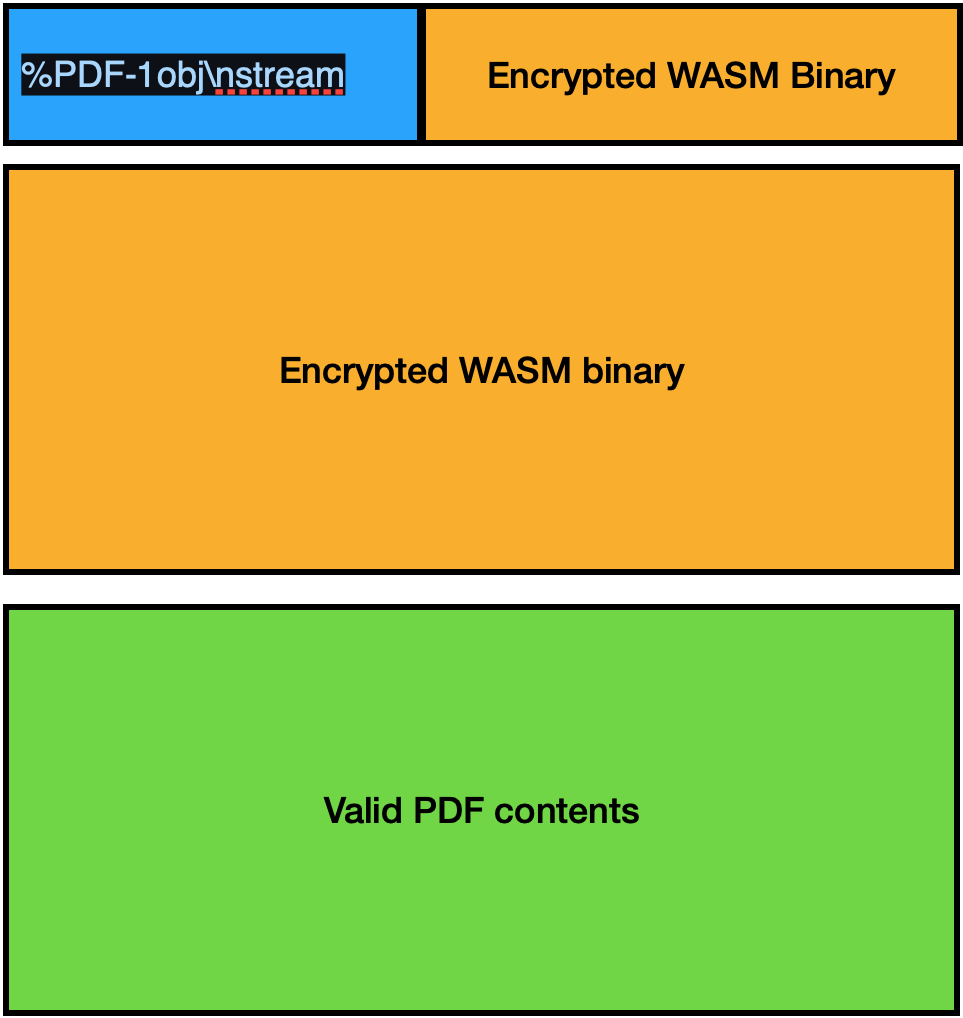
\includegraphics[width=8cm]{images/enc.png}
    \caption{Encryption Polyglot}
\end{figure}

The WASM binary has to follow certain rules to make this work. The last few bytes of the WASM binary needs to define a custom section with the length of the 
appended PDF contents encoded as LEB128. This is needed to make it so when we decrypt the file it will be a valid WASM binary as decryption yields random data for the
PDF contents and we don't care about them within the WASM binary so we wrap them inside a custom section.

\begin{figure}[h]
    \center
    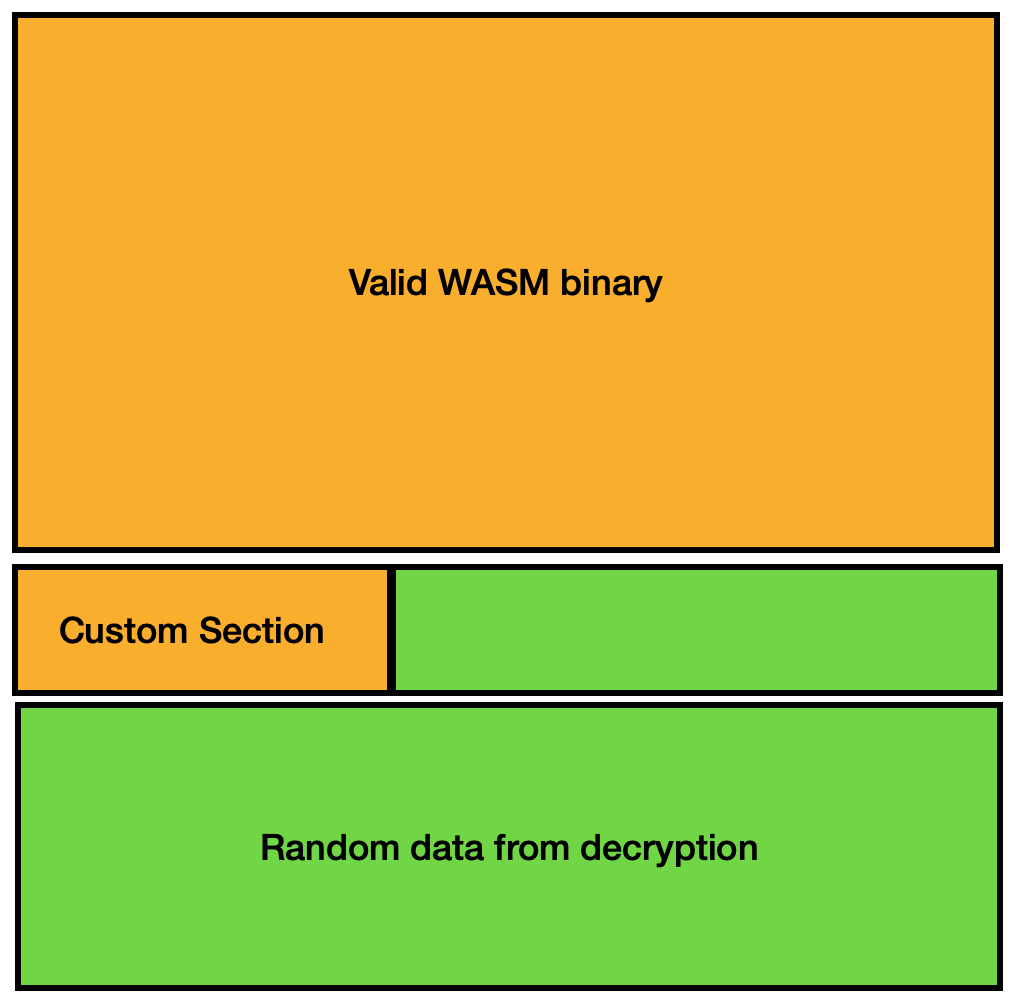
\includegraphics[width=8cm]{images/dec.png}
    \caption{Decrypting Polyglot}
\end{figure}

This is also possible with other file formats that have metadata or comment sections that we can use to hide data, such as PNG.
